\documentclass[landscape]{article}
\usepackage{amssymb}
\usepackage[landscape]{geometry}
\usepackage{multicol}
%\usepackage{helvet}
\usepackage{color}
%\usepackage[xdvi,dvips]{graphicx}
\usepackage{graphicx}
\usepackage{tikz}
\usepackage{amsfonts, amstext, amsmath}
\usepackage{wrapfig}
\usepackage{float}
\usepackage[export]{adjustbox}
\usepackage{tcolorbox}
\usepackage{times}
\usepackage{anyfontsize}
\usepackage{tikz}
\usepackage{graphicx}
\usetikzlibrary{calc,bayesnet,shapes.geometric,arrows,chains,matrix,positioning,scopes,calendar,decorations.markings,decorations.pathreplacing,intersections}

\makeatletter
\tikzset{join/.code=\tikzset{after node path={%
      \ifx\tikzchainprevious\pgfutil@empty\else(\tikzchainprevious)%
      edge[every join]#1(\tikzchaincurrent)\fi}}
}
\tikzset{>=stealth',every on chain/.append style={join},
  every join/.style={->}
}

\newcommand{\inputTikZ}[2]{%  
     \scalebox{#1}{\input{#2}}  
}

\newtcolorbox{mybox}{boxrule=6pt}

\def\argmax{\qopname\relax n{argmax}}
\def\s{\mathbf s}
\def\x{\mathbf x}
\def\u{\mathbf u}
\def\y{\mathbf y}
\def\d{\mathbf d}
\def\boldzero{\mathbf 0}
\def\pibold{\mbox{\boldmath $\pi$}}
\newcommand{\normal}[2]{\ensuremath{\mathcal{N}\left(#1,#2\right)}}
\newcommand{\given}{\mid}

\newenvironment{itemizeNoSymbol}{%
\renewcommand{\labelitemi}{}\begin{itemize}
\setlength{\itemsep}{1pt}
\setlength{\parskip}{0pt}
\setlength{\parsep}{0pt}}{\end{itemize}}


% set horizontal margins to center text (using current paperwidth &
% textwidth)
\newcommand{\equalmargins} {
\setlength{\oddsidemargin}{\paperwidth}
\addtolength{\oddsidemargin}{-\textwidth}
\setlength{\oddsidemargin}{0.5 \oddsidemargin}
\addtolength{\oddsidemargin}{-1in}
}

\setlength{\evensidemargin}{\oddsidemargin}

\renewcommand{\familydefault}{\sfdefault}

\input posterfonts.tex

% setup large (poster-sized) sheet
\setlength{\paperwidth}{841mm}
\setlength{\paperheight}{1189mm}
%\pdfpagewidth\paperwidth
%\pdfpageheight\paperheight
 
\setlength{\textwidth}{820mm}
\setlength{\textheight}{1170mm}
\setlength{\topmargin}{-.25truein}
 
\equalmargins
\setlength{\headsep}{0pt}
\setlength{\headheight}{0pt}

\pagestyle{empty}
\setlength{\parindent}{0mm}
\setlength{\parskip}{16pt}

% header style: title followed by a column-wide rule
\newcommand{\mysection}[1]{{\color[rgb]{.6,0,0}{\section*{{\huge #1}
        {\leaders\hrule height .2ex\hfill\kern0pt}}}}}

\begin{document}
\color{black}

% invisible rule is useful for spacing
\hrule width 0pt depth 0pt height 1pt

\begin{center}
  \HUGE
Approximating exponential family models \\ (not single distributions) with a two-network architecture \\
  \huge %
  Sean R. Bittner$^{1}$, John P. Cunningham$^2$ \\
  \LARGE
  $^{1}$Department of Neuroscience and $^{2}$Department of Statistics, Columbia University Medical Center
\end{center}

\begin{tikzpicture}[remember picture,overlay]
  \node[anchor=north east,inner sep=0pt, scale=0.35] at ($(current page.north east)+(+2.5cm,-1cm)$) {
     
\includegraphics{figs/CU_logo}
  };
\end{tikzpicture}

%%%%%%%%%%%%%%%%%%%%%%%%%%%%%%
\begin{minipage}[c]{0.28\linewidth}

\mysection{Motivation}
\large
\begin{itemize}
\item Variational inference (VI) incurs a cost of optimization to find optimal variational parameters $\theta^* \in \Theta$ of the approximate inference model.

\item Intractable exponential family models
\begin{itemize}
\item an exp fam likelihood
\item i.i.d. observations
\item a nonconjugate prior 
\end{itemize}
have a fixed-dimensionality natural parameterization $\eta$ with increased sampling.

\item If we can learn a smooth function $f_{\phi^*} : H \rightarrow \Theta$ mapping $\eta$ to $\theta^*$,

\begin{center}
\hspace{-1.0in}
\includegraphics[scale=1.0]{figs/amortizedVI/amortizedVI2.png}
\end{center}
there is potential for large savings through amortized variational inference.
\end{itemize}

\mysection{Methods}
{\huge \textbf{Background: topic}}
stuff
\begin{multicols*}{2}
\vspace{-1in}
column 1
\columnbreak
column 2
\end{multicols*}

 \inputTikZ{1}{figs/fig1/efn1b.tex} 
\end{minipage}
\begin{minipage}[c]{0.4\linewidth}
%%%%%%%%%%%%%%%%%%%%%%%%%%%%%%
\mysection{Application 1: 4-neuron V1 model}
\begin{center}
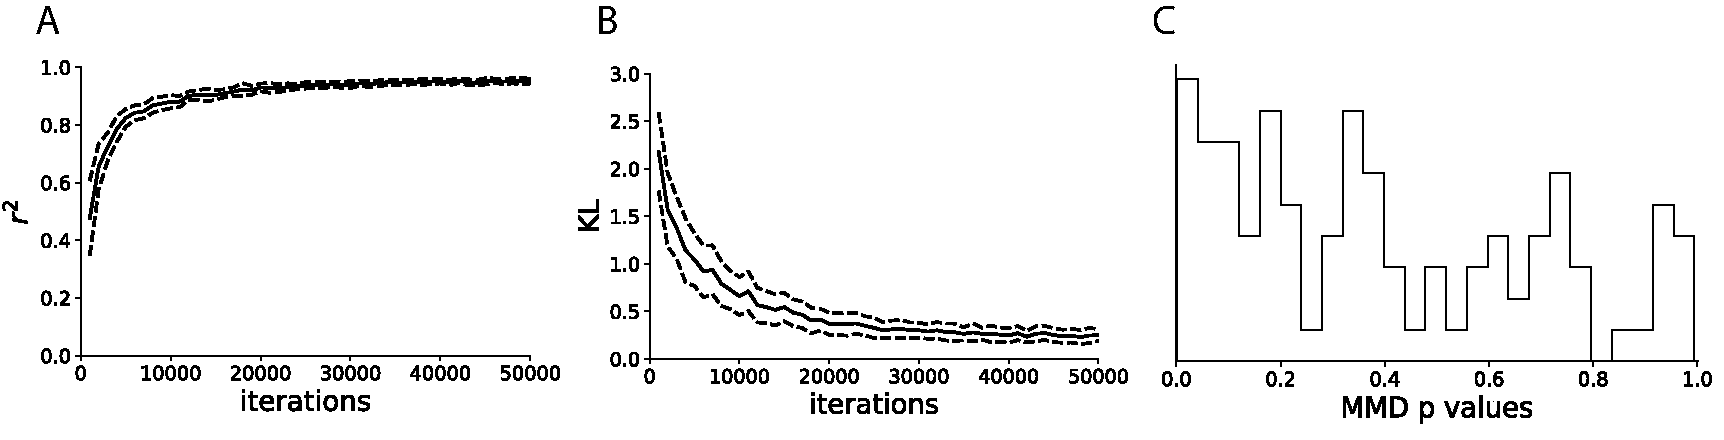
\includegraphics[scale=1.2]{figs/fig2/fig2.png}
\end{center}
{\LARGE \textbf{Emergent properties:}} \\

\begin{center}
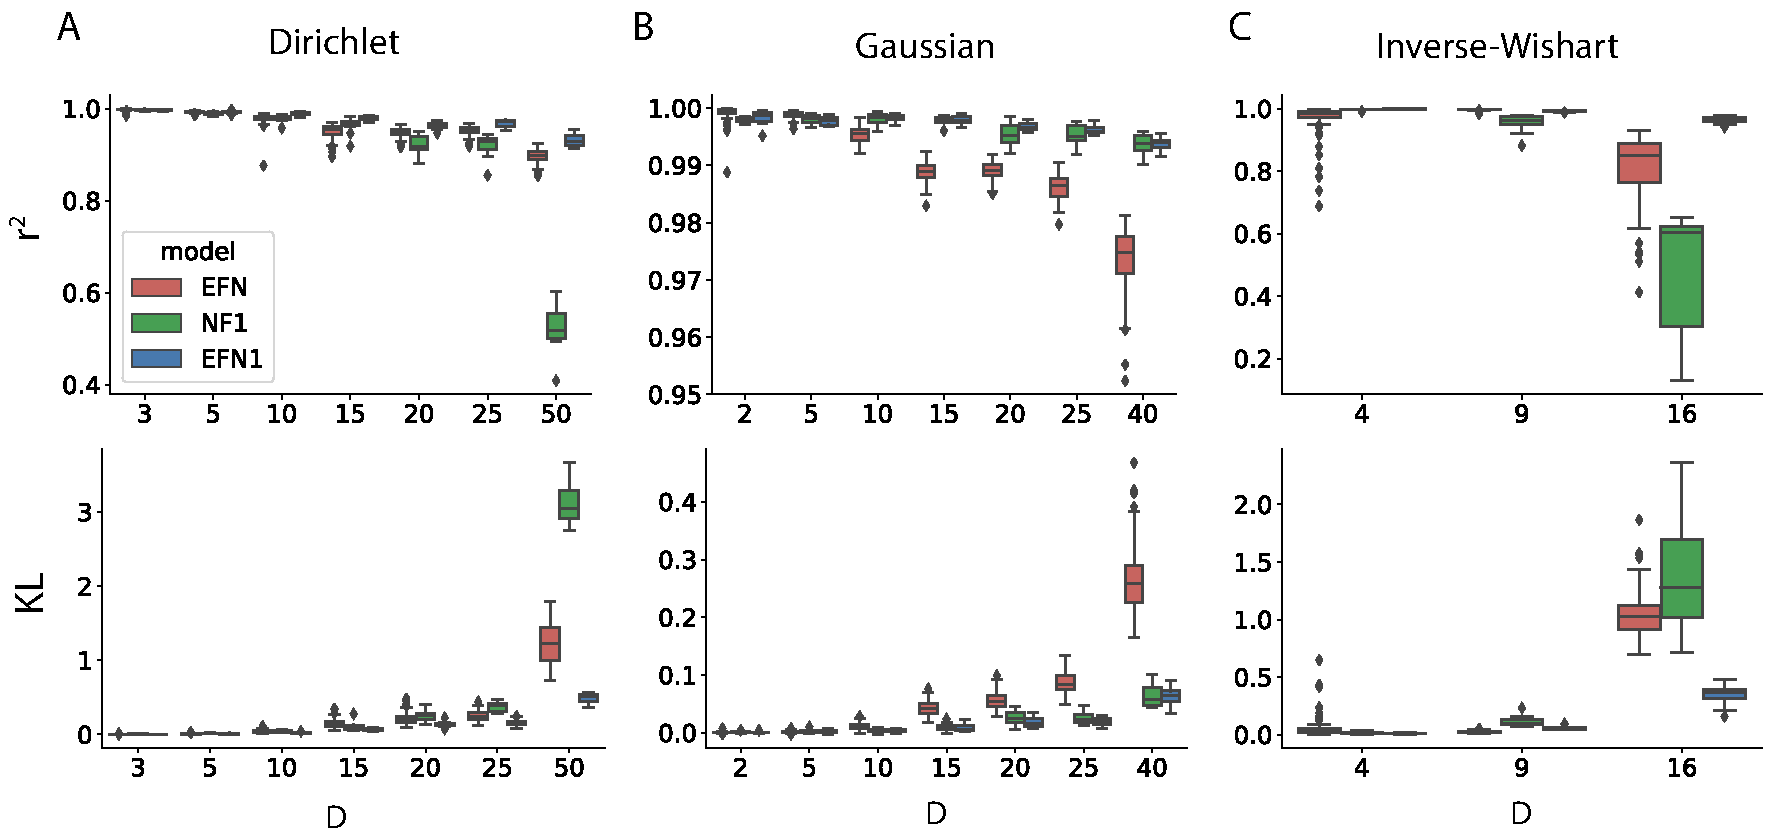
\includegraphics[scale=1.2]{figs/fig3/fig3.png}
\end{center}
\end{minipage}
\begin{minipage}[c]{0.28\linewidth}
%%%%%%%%%%%%%%%%%%%%%%%%%%%%%%
\mysection{More stuff}
\begin{center}
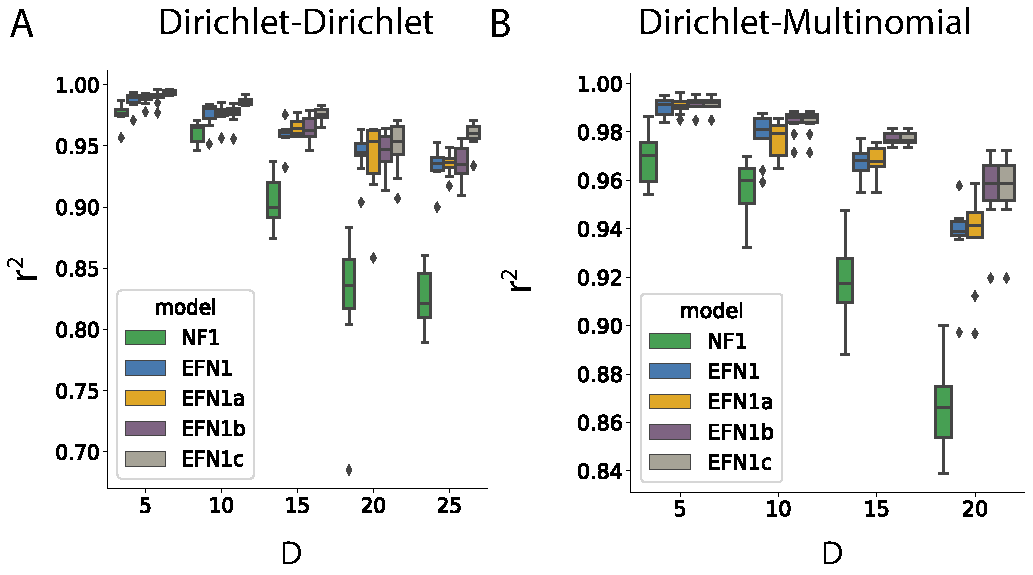
\includegraphics[scale=1.2]{figs/fig4/fig4.png}
\end{center}

\mysection{Summary}
\begin{itemize}
\item Summary point 1
\item Summary point 2
\end{itemize}


\large

{\bf\Large References}

1. Loaiza-Ganem, G., Y. Gao., and J. P. Cunningham. ``Maximum entropy flow networks." ICLR (2017). \\
2. Dipoppa, M., et al. ``Vision and locomotion shape the interactions between neuron types in mouse visual cortex." Neuron (2018). \\
3. Mastrogiuseppe, F., and S. Ostojic. ``Linking connectivity, dynamics, and computations in low-rank recurrent neural networks." Neuron (2018).

{\bf\Large Acknowledgements} \\
NSF Graduate Research Fellowship,  DGE-1644869, McKnight Endowment Fund, NIH NINDS 5R01NS100066, Simons Foundation 542963, NSF 1707398, The Gatsby Charitable Foundation \\

\end{minipage}
\end{document}
